\documentclass[11pt,a4paper]{article}
\usepackage[utf8]{inputenc}
\usepackage{amsmath,amsfonts,amssymb}
\usepackage{graphicx}
\usepackage{geometry}
\geometry{margin=1in}
\usepackage{booktabs}
\usepackage{hyperref}
\usepackage{float}
\usepackage{xcolor}

\definecolor{darkbg}{HTML}{0d121f}
\definecolor{lighttext}{HTML}{e2e8f0}
\definecolor{primary}{HTML}{8b5cf6}
\definecolor{secondary}{HTML}{0dd5c5}

\pagecolor{darkbg}
\color{lighttext}

\hypersetup{
    colorlinks=true,
    linkcolor=secondary,
    urlcolor=secondary
}

\title{\textbf{EE3621: Digital Signal Processing} \\ \Large Lecture 13: IIR Filter Structures --- Direct, Cascade \& Parallel Forms \\ \large (III B.Tech EEE)}
\author{Lecture Notes (40-Minute Plan)}
\date{}

\begin{document}

\maketitle

\section{Lecture Plan (40 Minutes Breakdown)}
\begin{itemize}
    \item \textbf{00:00 -- 05:00 (5 mins):} Welcome \& Introduction to IIR Systems. Transfer function, difference equations, and flow graph basic elements.
    \item \textbf{05:00 -- 12:00 (7 mins):} Direct Form I. Separate delay lines, node equations.
    \item \textbf{12:00 -- 18:00 (6 mins):} Direct Form II (Canonical Form). Combining delay lines, state equations, Transposed forms.
    \item \textbf{18:00 -- 25:00 (7 mins):} Cascade (Series) Form. Factoring into second-order sections (biquads).
    \item \textbf{25:00 -- 32:00 (7 mins):} Parallel Form. Partial fraction expansion.
    \item \textbf{32:00 -- 35:00 (3 mins):} Coefficient Sensitivity, Quantization Effects, Lattice-Ladder structures.
    \item \textbf{35:00 -- 40:00 (5 mins):} Checkpoints \& Numerical Examples.
\end{itemize}

\noindent\rule{\textwidth}{0.5pt}

\section{General IIR Transfer Function}
An Infinite Impulse Response (IIR) filter has a rational system function of the form:
\begin{equation}
H(z) = \frac{B(z)}{A(z)} = \frac{\sum_{k=0}^{M} b_k z^{-k}}{1 + \sum_{k=1}^{N} a_k z^{-k}}
\end{equation}
By dividing the output $Y(z)$ by the input $X(z)$:
\begin{equation}
\frac{Y(z)}{X(z)} = \frac{\sum_{k=0}^{M} b_k z^{-k}}{1 + \sum_{k=1}^{N} a_k z^{-k}}
\end{equation}
Cross-multiplying gives:
\begin{equation}
Y(z) \left( 1 + \sum_{k=1}^{N} a_k z^{-k} \right) = X(z) \left( \sum_{k=0}^{M} b_k z^{-k} \right)
\end{equation}
\begin{equation}
Y(z) + \sum_{k=1}^{N} a_k z^{-k} Y(z) = \sum_{k=0}^{M} b_k z^{-k} X(z)
\end{equation}
Isolating $Y(z)$:
\begin{equation}
Y(z) = \sum_{k=0}^{M} b_k z^{-k} X(z) - \sum_{k=1}^{N} a_k z^{-k} Y(z)
\end{equation}
Taking the inverse Z-transform yields the difference equation:
\begin{equation}
y[n] = \sum_{k=0}^{M} b_k x[n-k] - \sum_{k=1}^{N} a_k y[n-k]
\end{equation}
\textbf{Physical/Engineering Intuition:} The $b_k$ coefficients represent feedforward paths (zeros), and the $a_k$ coefficients represent feedback paths (poles).

\section{Direct Form I Structure}

\begin{figure}[H]
    \centering
    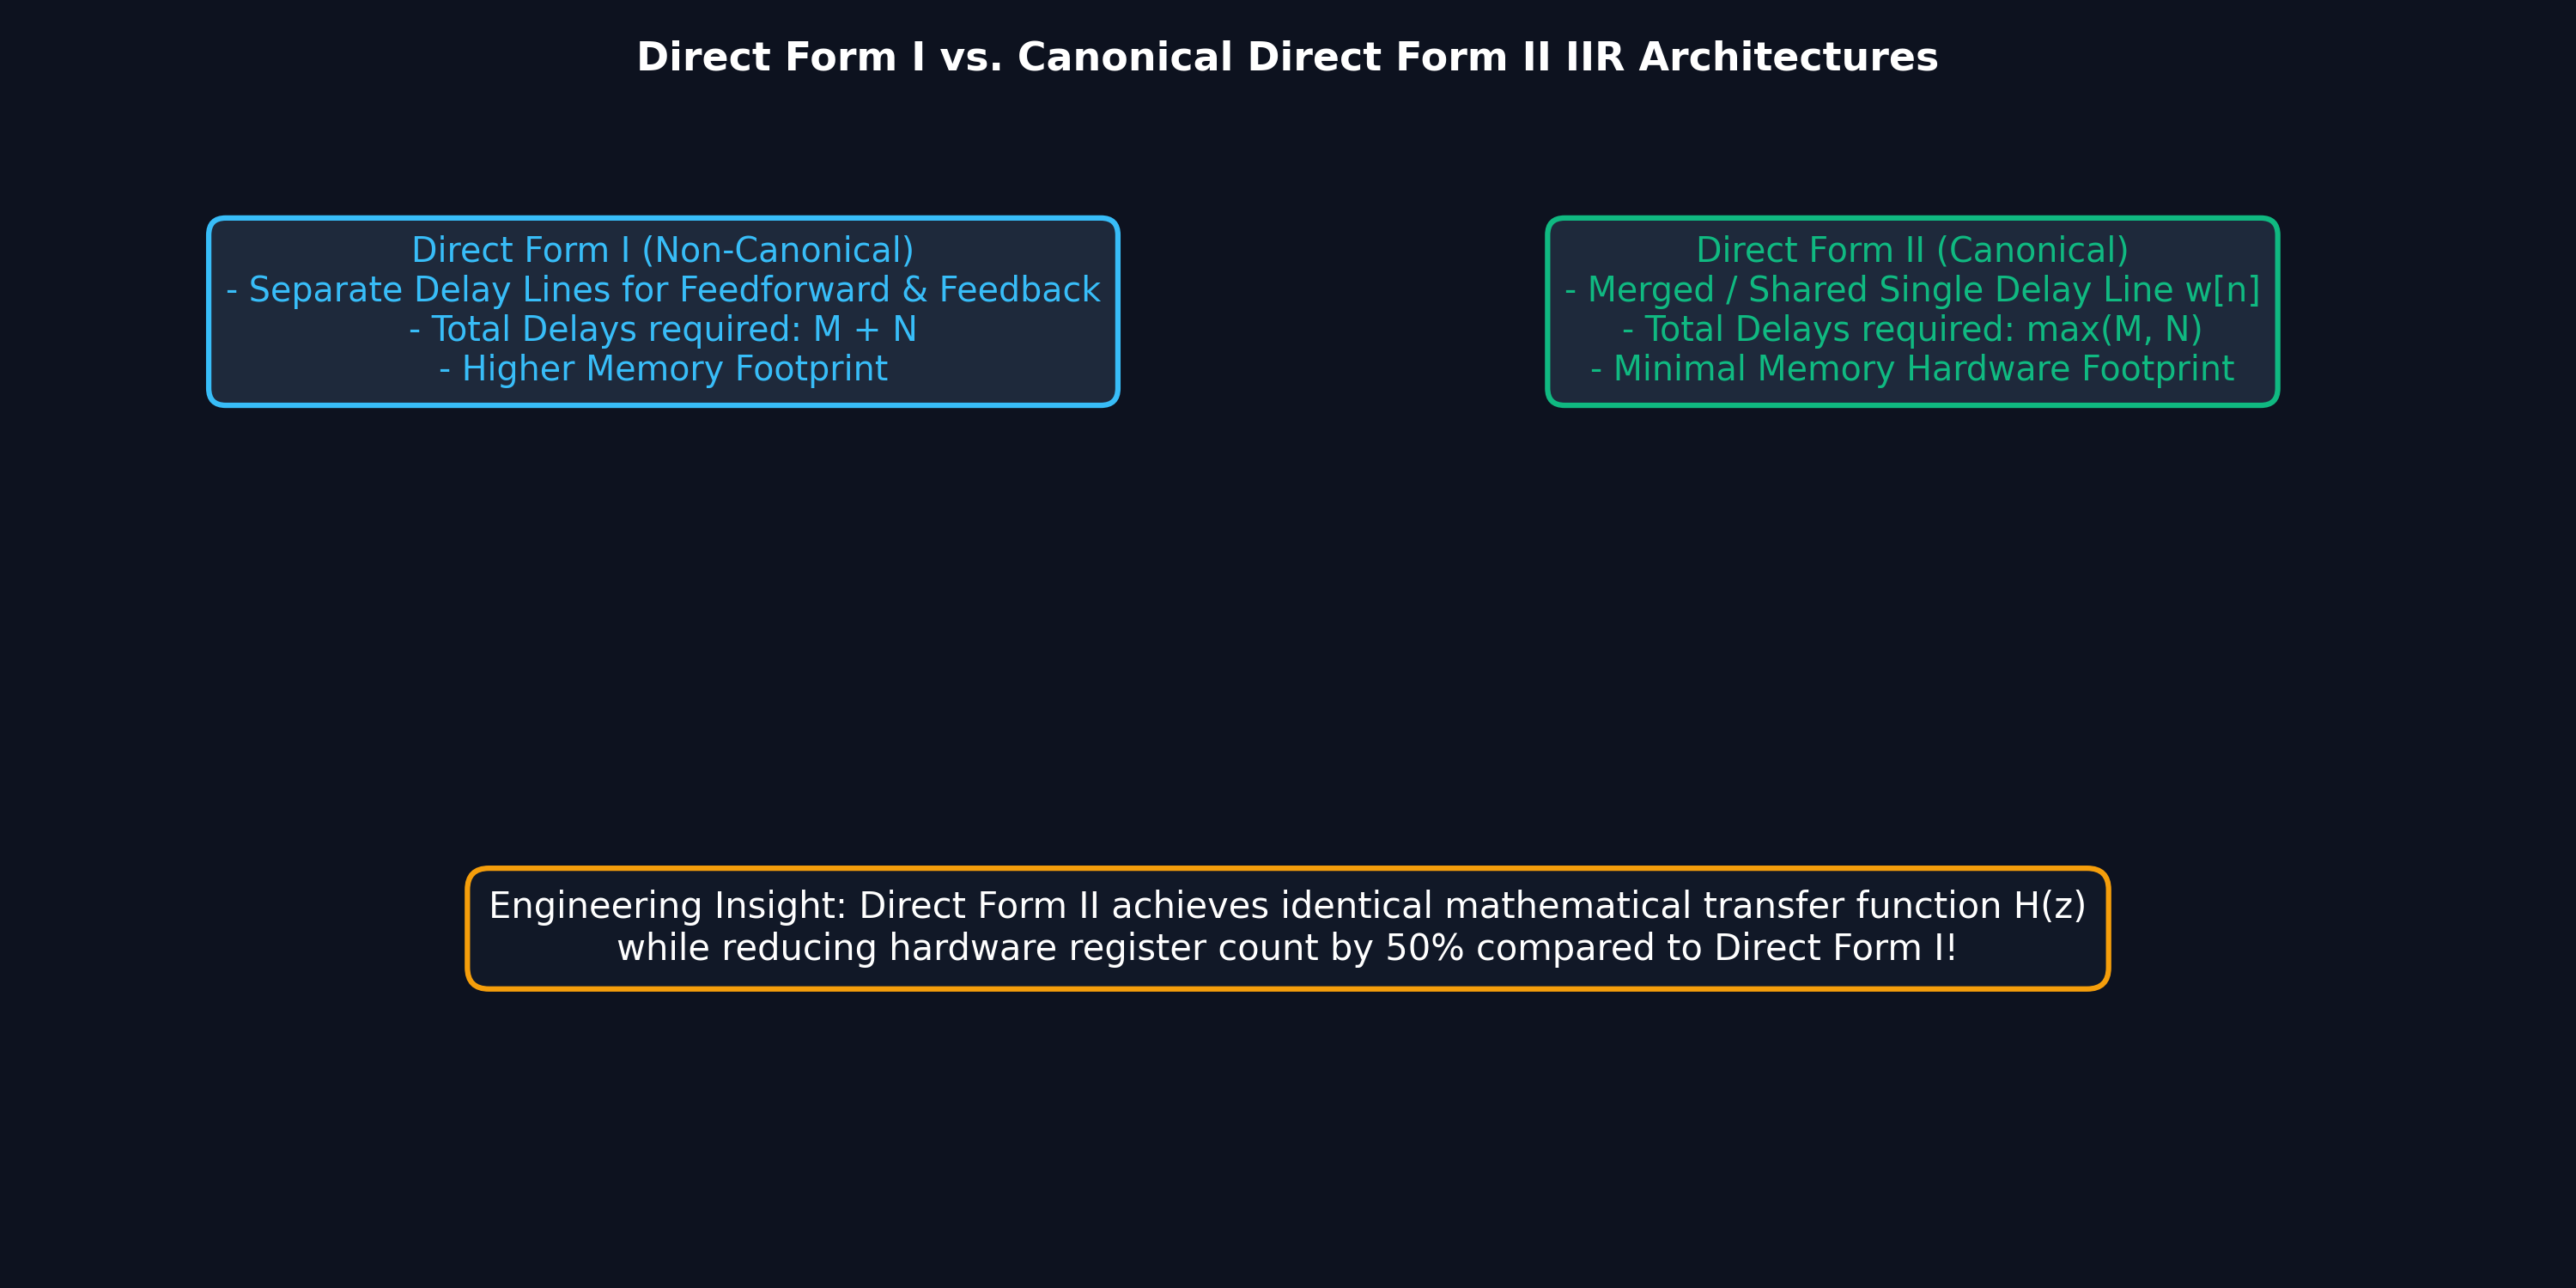
\includegraphics[width=0.85\textwidth]{images/iir_direct_form_i_ii_comparison.png}
    \caption{Direct Form I vs. Canonical Direct Form II: Achieving $50\%$ Delay Register Savings.}
\end{figure}

\begin{figure}[H]
    \centering
    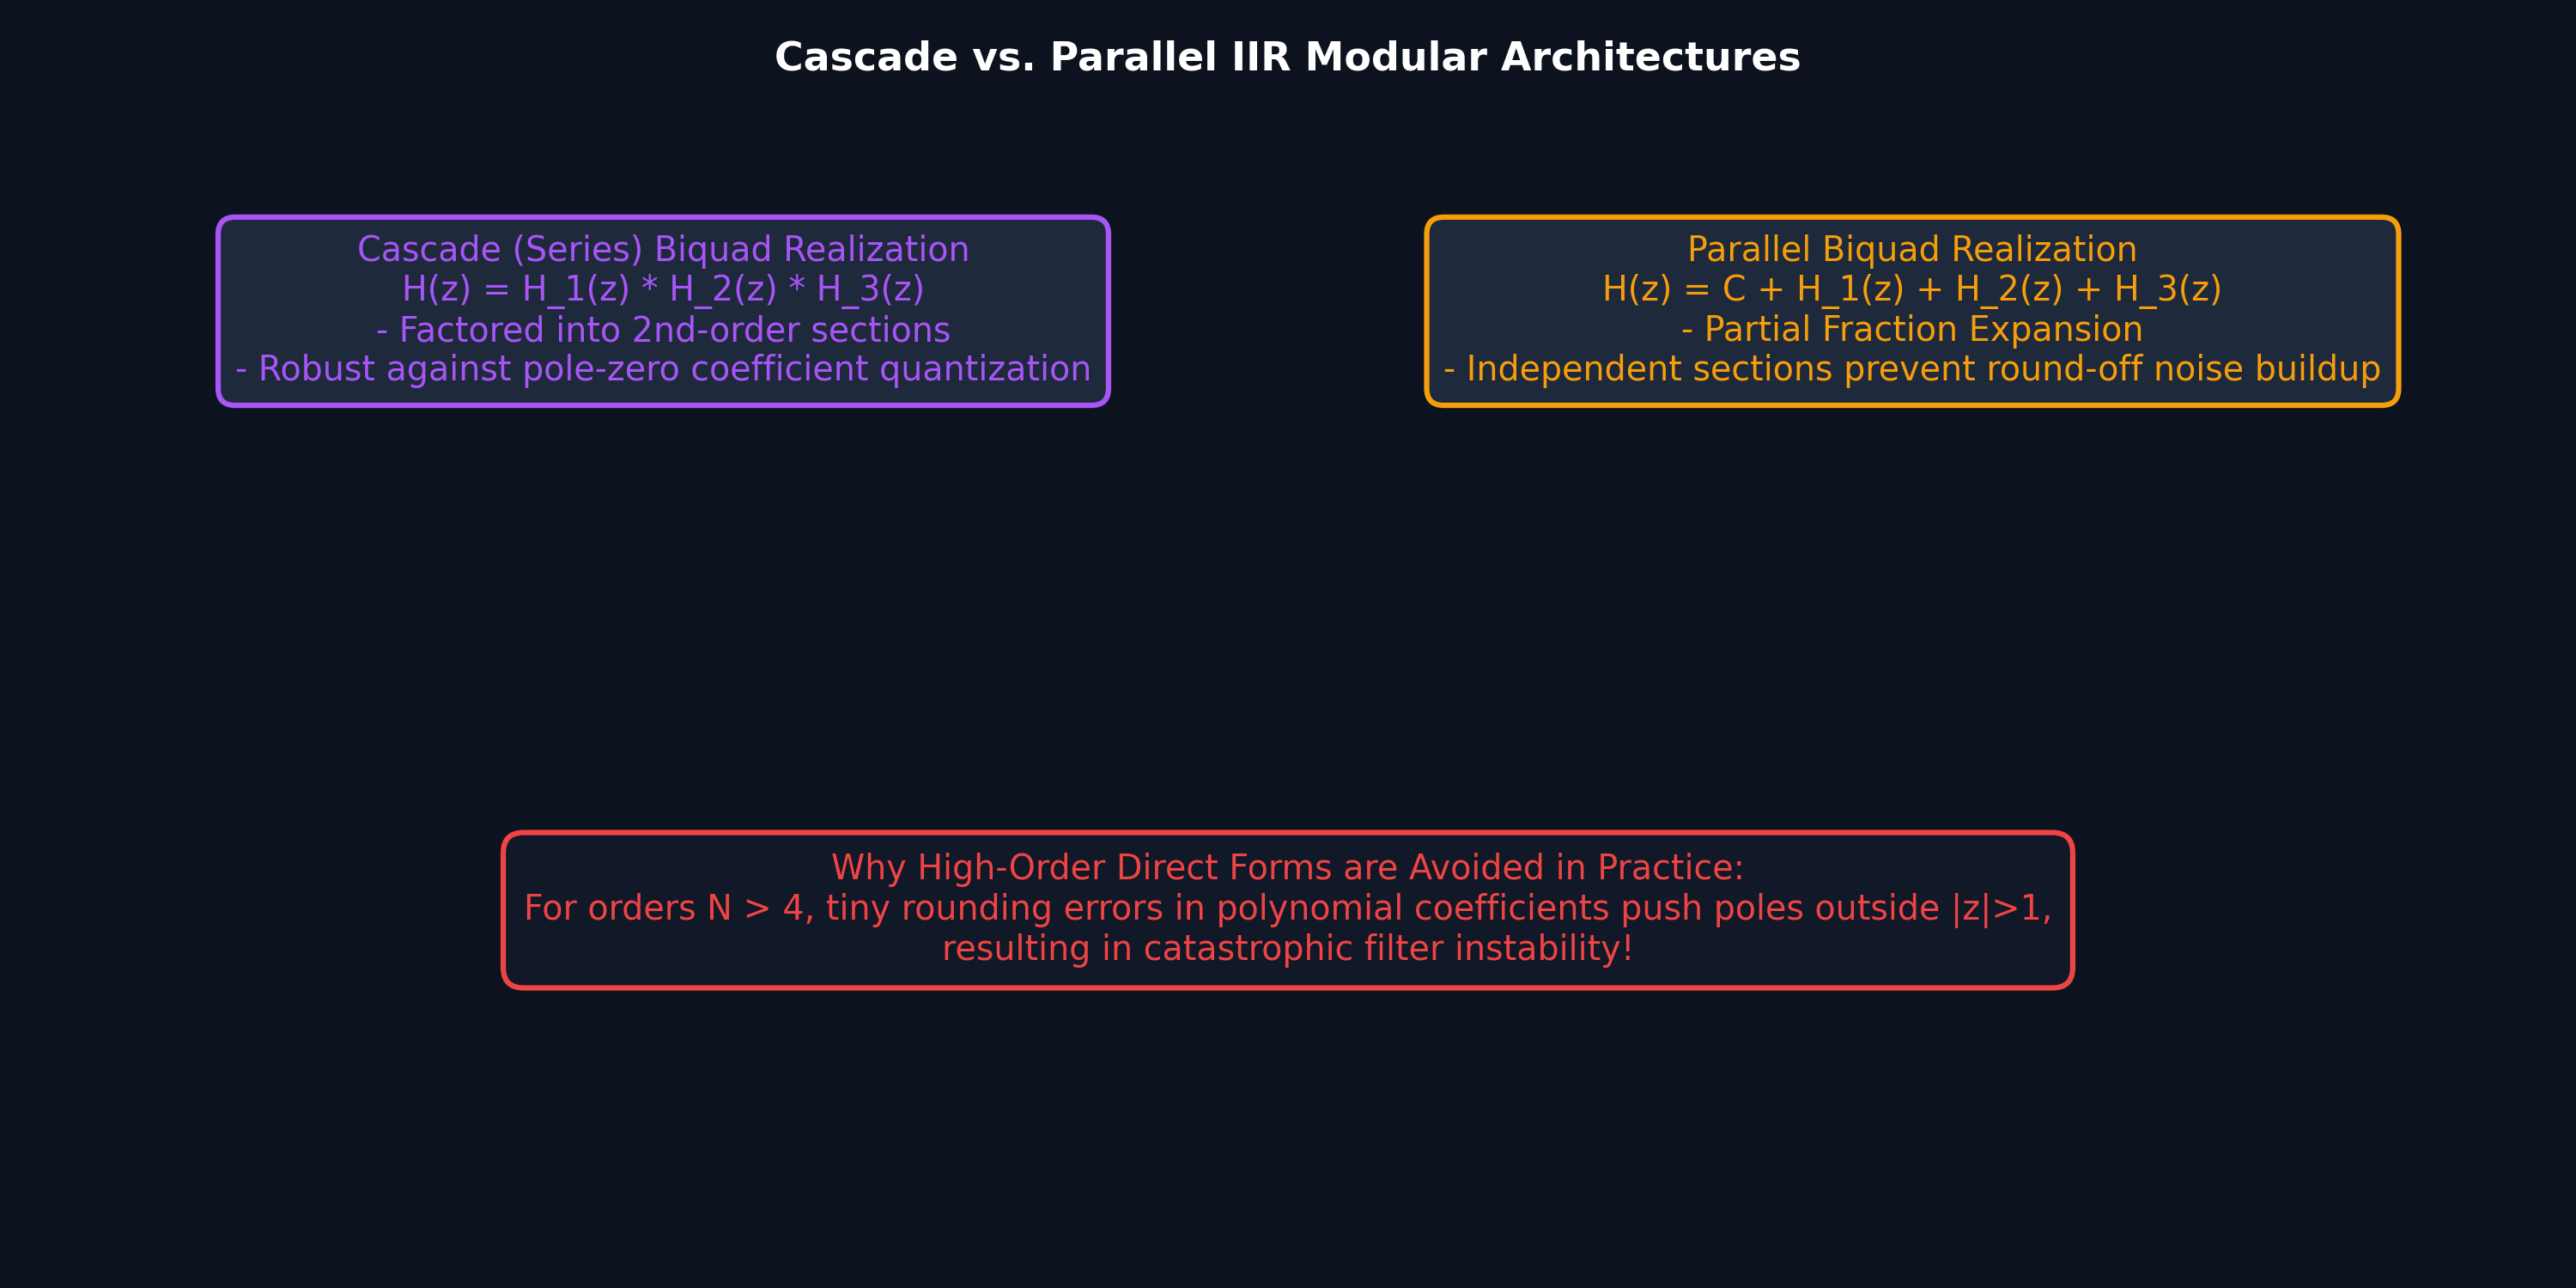
\includegraphics[width=0.85\textwidth]{images/iir_cascade_parallel_architectures.png}
    \caption{Cascade (Biquad Series) vs. Parallel Modular Architectures for Robust Fixed-Point Stability.}
\end{figure}


The Direct Form I structure implements the difference equation exactly as written. 
Let $w[n]$ be an intermediate sequence:
\begin{equation}
w[n] = \sum_{k=0}^{M} b_k x[n-k]
\end{equation}
Then the output $y[n]$ is:
\begin{equation}
y[n] = w[n] - \sum_{k=1}^{N} a_k y[n-k]
\end{equation}
\textbf{Memory Requirements:} Total memory elements = $M + N$. 

\section{Direct Form II (Canonical Form)}
We can swap the FIR and IIR parts because they are LTI:
\begin{equation}
H(z) = H_{IIR}(z) \cdot H_{FIR}(z) = \left( \frac{1}{1 + \sum_{k=1}^{N} a_k z^{-k}} \right) \cdot \left( \sum_{k=0}^{M} b_k z^{-k} \right)
\end{equation}
Let $V(z)$ be the output of the all-pole part:
\begin{equation}
V(z) = X(z) - \sum_{k=1}^{N} a_k z^{-k} V(z) \implies v[n] = x[n] - \sum_{k=1}^{N} a_k v[n-k]
\end{equation}
Now, pass $V(z)$ through the FIR part:
\begin{equation}
Y(z) = V(z) \cdot \left( \sum_{k=0}^{M} b_k z^{-k} \right) \implies y[n] = \sum_{k=0}^{M} b_k v[n-k]
\end{equation}
\textbf{Memory Requirements:} Total memory elements = $\max(M, N)$. This minimum memory form is the \textbf{Canonical Form}.

\section{Cascade (Series) Form}
To mitigate quantization errors, we factor $H(z)$ into 1st and 2nd-order sections (biquads).
\begin{equation}
H(z) = G \prod_{k=1}^{K} H_k(z) \quad \text{where} \quad H_k(z) = \frac{b_{k0} + b_{k1} z^{-1} + b_{k2} z^{-2}}{1 + a_{k1} z^{-1} + a_{k2} z^{-2}}
\end{equation}
Complex conjugate poles and zeros form real-coefficient biquads.

\section{Parallel Form}
Another decomposition uses Partial Fraction Expansion:
\begin{equation}
H(z) = C + \sum_{k=1}^{K} H_k(z) \quad \text{where} \quad H_k(z) = \frac{\gamma_{k0} + \gamma_{k1} z^{-1}}{1 + a_{k1} z^{-1} + a_{k2} z^{-2}}
\end{equation}

\section{Coefficient Sensitivity \& Quantization Effects}
High-order Direct Form I suffers from extreme root sensitivity to coefficient rounding. Cascade and parallel forms localize the errors to individual 2nd-order sections, maintaining filter stability.

\section{Lattice-Ladder structures}
Lattice-Ladder filters use reflection coefficients (PARCOR). An all-pole (AR) filter is strictly stable if and only if $|K_m| < 1$.

\section{Key Formulas}
\begin{table}[H]
\centering
\begin{tabular}{ll}
\toprule
\textbf{Concept} & \textbf{Equation / Transfer Function} \\
\midrule
Difference Equation & $y[n] = \sum_{k=0}^{M} b_k x[n-k] - \sum_{k=1}^{N} a_k y[n-k]$ \\
Direct Form II State Eq & $v[n] = x[n] - \sum_{k=1}^{N} a_k v[n-k]$; $y[n] = \sum_{k=0}^{M} b_k v[n-k]$ \\
Biquad Section (Cascade) & $H_k(z) = \frac{b_{k0} + b_{k1} z^{-1} + b_{k2} z^{-2}}{1 + a_{k1} z^{-1} + a_{k2} z^{-2}}$ \\
Parallel Section & $H_k(z) = \frac{\gamma_{k0} + \gamma_{k1} z^{-1}}{1 + a_{k1} z^{-1} + a_{k2} z^{-2}}$ \\
Stability via Lattice & $|K_m| < 1 \quad \forall m$ \\
\bottomrule
\end{tabular}
\end{table}

\section{Checkpoint Questions}
\begin{itemize}
    \item \textbf{Q1:} An IIR filter has $H(z) = \frac{1 + 2z^{-1} + z^{-2}}{1 - 0.5z^{-1} + 0.25z^{-2}}$. How many delay elements are required for Direct Form I vs Direct Form II? \\
    \textit{Answer:} Direct Form I: $M+N = 2+2=4$. Direct Form II: $\max(M,N) = 2$.
    \item \textbf{Q2:} Decompose $H(z) = \frac{1}{(1 - 0.5z^{-1})(1 - 0.25z^{-1})}$ into a Parallel Form. \\
    \textit{Answer:} Using PFE, $A = \frac{1}{1 - 0.25(2)} = 2$, $B = \frac{1}{1 - 0.5(4)} = -1$. $H(z) = \frac{2}{1 - 0.5z^{-1}} - \frac{1}{1 - 0.25z^{-1}}$.
    \item \textbf{Q3:} Why are Cascade/Parallel forms preferred over Direct Form I? \\
    \textit{Answer:} High-order polynomial roots are hypersensitive to coefficient quantization, causing instability. Lower-order forms localize errors.
\end{itemize}

\end{document}
